\section{Derivable and non-abstract
type}\label{derivable-and-non-abstract-type}

It is more common to make a non-abstract derivable type than abstract
type. This section covers how to make non-abstract derivable type
objects. A derivable type example is an object for string. It is TStr.
And its child is an object for numeric string. A numeric string is a
string that expresses a number. For example, ``0'', ``-100'' and
``123.45''. The child object (numeric string) will be explained in the
next section.

This section describes memory management for strings before derivable
objects.

\subsection{String and memory
management}\label{string-and-memory-management}

TStr has a string type value. It is similar to TInt or TDouble but
string is more complex than int and double. When you make TStr program,
you need to be careful about memory management, which is not necessary
to TInt and TDouble.

\subsubsection{String and memory}\label{string-and-memory}

String is an array of characters that is terminated with
`\textbackslash0'. String is not a C type such as char, int, float or
double. But the pointer to a character array behaves like a string type
of other languages. So, we often call the pointer string.

If the pointer is NULL, it points nothing. So, the pointer is not a
string. Programs with string will include bugs if you aren't careful
about NULL pointer.

Another annoying problem is memory allocation. Because string is an
array of characters, memory allocation is necessary to create a new
string. We don't forget to allocate memory, but often forget to free the
memory. It causes memory leak.

\begin{lstlisting}[language=C]
char *s;
s = g_strdup ("Hello.");
... ... ... do something with s
g_free (s);
\end{lstlisting}

\passthrough{\lstinline!g\_strdup!} duplicates a string. It does:

\begin{itemize}
\tightlist
\item
  Calculates the size of the string. The size of ``Hello.'' is 7 because
  strings are zero-terminated. The string is an array `H', `e', `l',
  `l', `o', `.' and zero (`\textbackslash0').
\item
  Requests the system to allocate 7 bytes memories.
\item
  Copies the string to the memory.
\item
  Returns the pointer to the newly-allocated memory.
\item
  If the argument is NULL, then no memory is allocated and it returns
  NULL.
\end{itemize}

If the string \passthrough{\lstinline!s!} is no longer in use,
\passthrough{\lstinline!s!} must be freed, which means the allocated 7
bytes must be returned to the system. \passthrough{\lstinline!g\_free!}
frees the memory.

Strings bounded by double quotes like ``Hello.'' are string literals.
They are an array of characters, but the contents of the array are not
allowed to change. And they mustn't be freed. If you write a character
in a string literal or free a string literal, the result is undefined.
Maybe bad things will happen, for example, a segmentation fault error.

There's a difference between arrays and pointers when you initialize
them with a string literal. If an array is initialized with a string
literal, the array can be changed.

\begin{lstlisting}[language=C]
char a[]="Hello!";
a[1]='a';
g_print ("%s\n", a); /* Hallo will appear on your display. */
\end{lstlisting}

The first line initializes an array \passthrough{\lstinline!a!}. The
initialization is not simple. First, the compiler calculates the length
of ``Hello!''. It is seven because the string literal has
`\textbackslash0' at the end of it. Then seven bytes memory is allocated
in static memory or stack memory. It depends on the class of the array,
whether \passthrough{\lstinline!static!} or
\passthrough{\lstinline!auto!}. The memory is initialized with
``Hello!''. So, the string in the array can be changed. This program
successfully displays `Hallo!.

The first line of the program above is the same as follows.

\begin{lstlisting}[language=C]
char a[] = {'H', 'e', 'l', 'l', 'o', '!', '\0'};
\end{lstlisting}

If you define a pointer with string literal, you can't change the string
pointed by the pointer.

\begin{lstlisting}[language=C]
char *a = "Hello";
*(a+1) = 'a'; /* This is illegal. */
g_print ("%s\n", a);
\end{lstlisting}

The first line just assigns the address of the string literal to the
variable \passthrough{\lstinline!a!}. String literal is an array of
characters but it's read-only. It might be in the program code area or
some other non-writable area. It depends on the implementation of your
compiler. Therefore, the second line tries to write a char `a' to the
read-only memory and the result is undefined, for example, a
segmentation error happens. Anyway, don't write a program like this.

In conclusion, a string is an array of characters and it is placed in
one of the following.

\begin{itemize}
\tightlist
\item
  Read-only memory. A string literal is read-only.
\item
  Stack. If the class of an array is \passthrough{\lstinline!auto!},
  then the array is placed in the stack. stack is writable. If the array
  is defined in a function, its default class is
  \passthrough{\lstinline!auto!}. The stack area will disappear when the
  function returns to the caller.
\item
  Static area. If the class of an array is
  \passthrough{\lstinline!static!}, then the array is placed in the
  static area. It keeps its value and remains for the life of the
  program. This area is writable.
\item
  Heap. You can allocate and free memory for a string. For allocation,
  \passthrough{\lstinline!g\_new!} or \passthrough{\lstinline!g\_new0!}
  is used. For freeing, \passthrough{\lstinline!g\_free!} is used.
\end{itemize}

\subsubsection{Copying string}\label{copying-string}

There are two ways to copy a string. First way is just copying the
pointer.

\begin{lstlisting}[language=C]
char *s = "Hello";
char *t = s;
\end{lstlisting}

Two pointers \passthrough{\lstinline!s!} and \passthrough{\lstinline!t!}
points the same address. Therefore, you can't modify
\passthrough{\lstinline!t!} because \passthrough{\lstinline!t!} points a
string literal, which is read-only.

Second way is creating memory and copying the string to the memory.

\begin{lstlisting}[language=C]
char *s = "Hello";
char *t = g_strdup (s);
\end{lstlisting}

The function \passthrough{\lstinline!g\_strdup!} allocates memory and
initializes it with ``Hello'', then returns the pointer to the memory.
The function \passthrough{\lstinline!g\_strdup!} is almost same as the
function \passthrough{\lstinline!string\_dup!} below.

\begin{lstlisting}[language=C]
#include <glib-object.h>
#include <string.h>

char *
string_dup (char *s) {
  int length;
  char *t;

  if (s == NULL)
    return NULL;
  length = strlen (s) + 1;
  t = g_new (char, length);
  strcpy (t, s);
  return t;
}
\end{lstlisting}

If \passthrough{\lstinline!g\_strdup!} is used, the two pointers
\passthrough{\lstinline!s!} and \passthrough{\lstinline!t!} point
different memories. You can modify \passthrough{\lstinline!t!} because
it is placed in the memory allocated from the heap area.

It is important to know the difference between assigning pointers and
duplicating strings.

\subsubsection{const qualifier}\label{const-qualifier}

The qualifier \passthrough{\lstinline!const!} makes a variable won't
change its value. It can also be applied to an array. Then, the elements
of the array won't be changed.

\begin{lstlisting}[language=C]
const double pi = 3.1415926536;
const char a[] = "read only string";
\end{lstlisting}

An array parameter in a function can be qualified with
\passthrough{\lstinline!const!} to indicate that the function does not
change the array. In the same way, the return value (a pointer to an
array or string) of a function can be qualified with
\passthrough{\lstinline!const!}. The caller mustn't modify or free the
returned array or string.

\begin{lstlisting}[language=C]
char *
string_dup (const char *s) {
  ... ...
}

const char *
g_value_get_string (const GValue *value);
\end{lstlisting}

The qualifier \passthrough{\lstinline!const!} indicates who is the owner
of the string when it is used in the function of objects. ``Owner'' is
an object or a caller of the function that has the right to modify or
free the string.

For example, \passthrough{\lstinline!g\_value\_get\_string!} is given
\passthrough{\lstinline!const GValue *value!} as an argument. The GValue
pointed by \passthrough{\lstinline!value!} is owned by the caller and
the function doesn't change or free it. The function returns a string
qualified with \passthrough{\lstinline!const!}. The returned string is
owned by the object and the caller mustn't change or free the string. It
is possible that the string will be changed or freed by the object
later.

\subsection{Header file}\label{header-file}

The rest of this section is about TStr. TStr is a child of GObject and
it holds a string. The string is a pointer and an array of characters.
The pointer points the array. The pointer can be NULL. If it is NULL,
TStr has no array. The memory of the array comes from the heap area.
TStr owns the memory and is responsible to free it when it becomes
useless. TStr has a string type property.

The header file \passthrough{\lstinline!tstr.h!} is as follows.

\begin{lstlisting}[language=C, numbers=left]
#pragma once

#include <glib-object.h>

#define T_TYPE_STR  (t_str_get_type ())
G_DECLARE_DERIVABLE_TYPE (TStr, t_str, T, STR, GObject)

struct _TStrClass {
  GObjectClass parent_class;
  /* expect that descendants will override the setter */
  void (*set_string)  (TStr *self, const char *s);
};

TStr *
t_str_concat (TStr *self, TStr *other);

/* setter and getter */
void
t_str_set_string (TStr *self, const char *s);

char *
t_str_get_string (TStr *self);

/* create a new TStr instance */
TStr *
t_str_new_with_string (const char *s);

TStr *
t_str_new (void);
\end{lstlisting}

\begin{itemize}
\tightlist
\item
  6: Uses \passthrough{\lstinline!G\_DECLARE\_DERIVABLE\_TYPE!}. The
  TStr class is derivable and its child class will be defined later.
\item
  8-12: TStrClass has one class method. It is
  \passthrough{\lstinline!set\_string!} member of the TStrClass
  structure. This will be overridden by the child class
  \passthrough{\lstinline!TNumStr!}. Therefore, Both TStr and TNumStr
  has \passthrough{\lstinline!set\_string!} member in their classes but
  they point different functions.
\item
  14-15: The public function \passthrough{\lstinline!t\_str\_concat!}
  connects two strings of TStr instances and returns a new TStr
  instance.
\item
  18-22: Setter and getter.
\item
  25-29: Functions to create a TStr object.
\end{itemize}

\subsection{C file}\label{c-file}

The C file \passthrough{\lstinline!tstr.c!} for TStr is as follows.

\begin{lstlisting}[language=C, numbers=left]
#include "tstr.h"

enum {
  PROP_0,
  PROP_STRING,
  N_PROPERTIES
};

static GParamSpec *str_properties[N_PROPERTIES] = {NULL, };

typedef struct {
  char *string;
} TStrPrivate;

G_DEFINE_TYPE_WITH_PRIVATE(TStr, t_str, G_TYPE_OBJECT)

static void
t_str_set_property (GObject *object, guint property_id, const GValue *value, GParamSpec *pspec) {
  TStr *self = T_STR (object);

/* The returned value of the function g_value_get_string can be NULL. */
/* The function t_str_set_string calls a class method, */
/* which is expected to rewrite in the descendant object. */
  if (property_id == PROP_STRING)
    t_str_set_string (self, g_value_get_string (value));
  else
    G_OBJECT_WARN_INVALID_PROPERTY_ID (object, property_id, pspec);
}

static void
t_str_get_property (GObject *object, guint property_id, GValue *value, GParamSpec *pspec) {
  TStr *self = T_STR (object);
  TStrPrivate *priv = t_str_get_instance_private (self);

/* The second argument of the function g_value_set_string can be NULL. */
  if (property_id == PROP_STRING)
    g_value_set_string (value, priv->string);
  else
    G_OBJECT_WARN_INVALID_PROPERTY_ID (object, property_id, pspec);
}

/* This function just set the string. */
/* So, no notify signal is emitted. */
static void
t_str_real_set_string (TStr *self, const char *s) {
  TStrPrivate *priv = t_str_get_instance_private (self);

  if (priv->string)
    g_free (priv->string);
  priv->string = g_strdup (s);
}

static void
t_str_finalize (GObject *object) {
  TStr *self = T_STR (object);
  TStrPrivate *priv = t_str_get_instance_private (self);

  if (priv->string)
    g_free (priv->string);
  G_OBJECT_CLASS (t_str_parent_class)->finalize (object);
}

static void
t_str_init (TStr *self) {
  TStrPrivate *priv = t_str_get_instance_private (self);

  priv->string = NULL;
}

static void
t_str_class_init (TStrClass *class) {
  GObjectClass *gobject_class = G_OBJECT_CLASS (class);

  gobject_class->finalize = t_str_finalize;
  gobject_class->set_property = t_str_set_property;
  gobject_class->get_property = t_str_get_property;
  str_properties[PROP_STRING] = g_param_spec_string ("string", "str", "string", "", G_PARAM_READWRITE);
  g_object_class_install_properties (gobject_class, N_PROPERTIES, str_properties);

  class->set_string = t_str_real_set_string;
}

/* setter and getter */
void
t_str_set_string (TStr *self, const char *s) {
  g_return_if_fail (T_IS_STR (self));
  TStrClass *class = T_STR_GET_CLASS (self);

/* The setter calls the class method 'set_string', */
/* which is expected to be overridden by the descendant TNumStr. */
/* Therefore, the behavior of the setter is different between TStr and TNumStr. */
  class->set_string (self, s);
}

char *
t_str_get_string (TStr *self) {
  g_return_val_if_fail (T_IS_STR (self), NULL);
  TStrPrivate *priv = t_str_get_instance_private (self);

  return g_strdup (priv->string);
}

TStr *
t_str_concat (TStr *self, TStr *other) {
  g_return_val_if_fail (T_IS_STR (self), NULL);
  g_return_val_if_fail (T_IS_STR (other), NULL);

  char *s1, *s2, *s3;
  TStr *str;

  s1 = t_str_get_string (self);
  s2 = t_str_get_string (other);
  if (s1 && s2)
    s3 = g_strconcat (s1, s2, NULL);
  else if (s1)
    s3 = g_strdup (s1);
  else if (s2)
    s3 = g_strdup (s2);
  else
    s3 = NULL;
  str = t_str_new_with_string (s3);
  if (s1) g_free (s1);
  if (s2) g_free (s2);
  if (s3) g_free (s3);
  return str;
}

/* create a new TStr instance */
TStr *
t_str_new_with_string (const char *s) {
  return T_STR (g_object_new (T_TYPE_STR, "string", s, NULL));
}

TStr *
t_str_new (void) {
  return T_STR (g_object_new (T_TYPE_STR, NULL));
}
\end{lstlisting}

\begin{itemize}
\tightlist
\item
  3-9: \passthrough{\lstinline!enum!} defines a property id. The member
  \passthrough{\lstinline!PROP\_STRING!} is the id of the ``string''
  property. Only one property is defined here, so it is possible to
  define it without \passthrough{\lstinline!enum!}. However,
  \passthrough{\lstinline!enum!} can be applied to define two or more
  properties and it is more common. The last member
  \passthrough{\lstinline!N\_PROPERTIES!} is two because
  \passthrough{\lstinline!enum!} is zero-based. An array
  \passthrough{\lstinline!str\_properties!} has two elements since
  \passthrough{\lstinline!N\_PROPERTIES!} is two. The first element
  isn't used and it is assigned with NULL. The second element will be
  assigned a pointer to a GParamSpec instance in the class
  initialization function.
\item
  11-13: TStrPrivate is a C structure. It is a private data area for
  TStr. If TStr were a final type, then no descendant would exist and
  TStr instance could be a private data area. But TStr is derivable so
  you can't store such private data in TStr instance that is open to the
  descendants. The name of this structure is ``\textless object
  name\textgreater Private'' like \passthrough{\lstinline!TStrPrivate!}.
  The structure must be defined before
  \passthrough{\lstinline!G\_DEFINE\_TYPE\_WITH\_PRIVATE!}.
\item
  15: \passthrough{\lstinline!G\_DEFINE\_TYPE\_WITH\_PRIVATE!} macro. It
  is similar to \passthrough{\lstinline!G\_DEFINE\_TYPE!} macro but it
  adds the private data area for the derivable instance. This macro
  expands to:

  \begin{itemize}
  \tightlist
  \item
    Declaration of \passthrough{\lstinline!t\_str\_class\_init!} which
    is a class initialization function.
  \item
    Declaration of \passthrough{\lstinline!t\_str\_init!} which is an
    instance initialization function.
  \item
    Definition of \passthrough{\lstinline!t\_str\_parent\_class!} static
    variable. It points to the parent class of TStr.
  \item
    The function call that adds private instance data to the type. It is
    a C structure and its name is \passthrough{\lstinline!TStrPrivate!}.
  \item
    Definition of \passthrough{\lstinline!t\_str\_get\_type ()!}
    function. This function registers the type in its first call.
  \item
    Definition of the private instance getter
    \passthrough{\lstinline!t\_str\_get\_instance\_private ()!}.
  \end{itemize}
\item
  17-28: The function \passthrough{\lstinline!t\_str\_set\_property!}
  sets the ``string'' property and it is used by
  \passthrough{\lstinline!g\_object\_set!} family functions. It uses
  \passthrough{\lstinline!t\_str\_set\_string!} function to set the
  private data with the copy of the string from the GValue. It is
  important because \passthrough{\lstinline!t\_str\_set\_string!} calls
  the class method \passthrough{\lstinline!set\_string!}, which will be
  overridden by the child class. Therefore, the behavior of
  \passthrough{\lstinline!t\_str\_set\_property!} function is different
  between TStr and TNumStr, which is a child of TStr. The function
  \passthrough{\lstinline!g\_value\_get\_string!} returns the pointer to
  the string that GValue owns. So you need to duplicate the string and
  it is done in the function
  \passthrough{\lstinline!t\_str\_set\_string!}.
\item
  30-40: The function \passthrough{\lstinline!t\_str\_get\_property!}
  gets the ``string'' property and it is used by
  \passthrough{\lstinline!g\_object\_get!} family functions. It just
  gives \passthrough{\lstinline!priv->string!} to the function
  \passthrough{\lstinline!g\_value\_set\_string!}. The variable
  \passthrough{\lstinline!priv!} points the private data area. The
  second argument \passthrough{\lstinline!priv->string!} is owned by the
  TStr instance and the function
  \passthrough{\lstinline!g\_value\_set\_string!} duplicates it to store
  in the GValue structure.
\item
  44-51 The function \passthrough{\lstinline!t\_str\_real\_set\_string!}
  is the body of the class method and pointed by
  \passthrough{\lstinline!set\_string!} member in the class. First, it
  gets the pointer to the private area with
  \passthrough{\lstinline!t\_str\_get\_instance\_private!} function. If
  the instance holds a string, free it before setting it to a new
  string. It copies the given string and assigns it to
  \passthrough{\lstinline!priv->string!}. The duplication is important.
  Thanks to that, the address of the string is hidden from the out of
  the instance.
\item
  53-61: The finalize function
  \passthrough{\lstinline!t\_str\_finalize!} is called when TStr
  instance is destroyed. The destruction process has two phases,
  ``dispose'' and ``finalize''. In the disposal phase, the instance
  releases instances. In the finalization phase, the instance does the
  rest of all the finalization like freeing memories. This function
  frees the string \passthrough{\lstinline!priv->string!} if necessary.
  After that, it calls the parent's finalize method. This is called
  ``chain up to its parent'' and it will be explained later in this
  section.
\item
  63-68: The instance initialization function
  \passthrough{\lstinline!t\_str\_init!} assigns NULL to
  \passthrough{\lstinline!priv->string!}.
\item
  70-81: The class initialization function
  \passthrough{\lstinline!t\_str\_class\_init!} overrides
  \passthrough{\lstinline!finalize!},
  \passthrough{\lstinline!set\_property!} and
  \passthrough{\lstinline!get\_property!} members. It creates the
  GParamSpec instance with
  \passthrough{\lstinline!g\_param\_spec\_string!} and installs the
  property with
  \passthrough{\lstinline!g\_object\_class\_install\_properties!}. It
  assigns \passthrough{\lstinline!t\_str\_real\_set\_string!} to the
  member \passthrough{\lstinline!set\_string!}. It is a class method and
  is expected to be replaced in the child class.
\item
  84-101: Setter and getter. The setter method
  \passthrough{\lstinline!t\_str\_set\_string!} just calls the class
  method. So, it is expected to be replaced in the child class. It is
  used by property set function
  \passthrough{\lstinline!t\_str\_set\_property!}. So the behavior of
  property setting will change in the child class. The getter method
  \passthrough{\lstinline!t\_str\_get\_string!} just duplicates the
  string \passthrough{\lstinline!priv->string!} and return the copy.
\item
  103-126: The public function \passthrough{\lstinline!t\_str\_concat!}
  concatenates the string of \passthrough{\lstinline!self!} and
  \passthrough{\lstinline!other!}, and creates a new TStr.
\item
  129-137: Two functions
  \passthrough{\lstinline!t\_str\_new\_with\_string!} and
  \passthrough{\lstinline!t\_str\_new!} create a new TStr instances.
\end{itemize}

\subsection{Chaining up to its parent}\label{chaining-up-to-its-parent}

The ``chain up to its parent'' process is illustrated with the diagram
below.

\begin{figure}
\centering
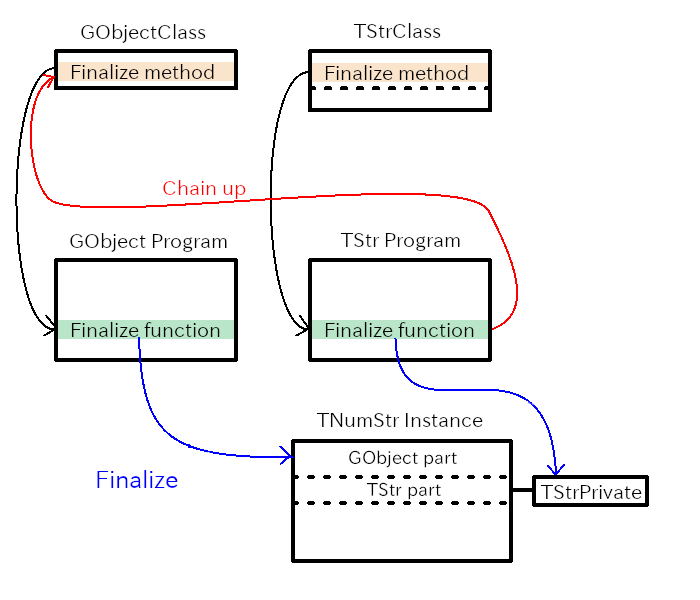
\includegraphics[width=10.5cm,height=9cm]{../image/chainup.png}
\caption{Chaining up process in GObject and TStr}
\end{figure}

There are two classes, GObjectClass and TStrClass. Each class has their
finalize methods (functions) pointed by the pointers in the class
structures. The finalize method of TStrClass finalizes its own part of
the TStr instance. At the end of the function, it calls its parent's
finalize method. It is the finalize method of GObjectClass. It calls its
own finalize function and finalizes the GObject private data.

If the GObjectClass has two or more descendant classes, the number of
the finalize functions may be the same as the number of the descendants.
And they are connected by ``chain up to its parent'' way.

\begin{figure}
\centering
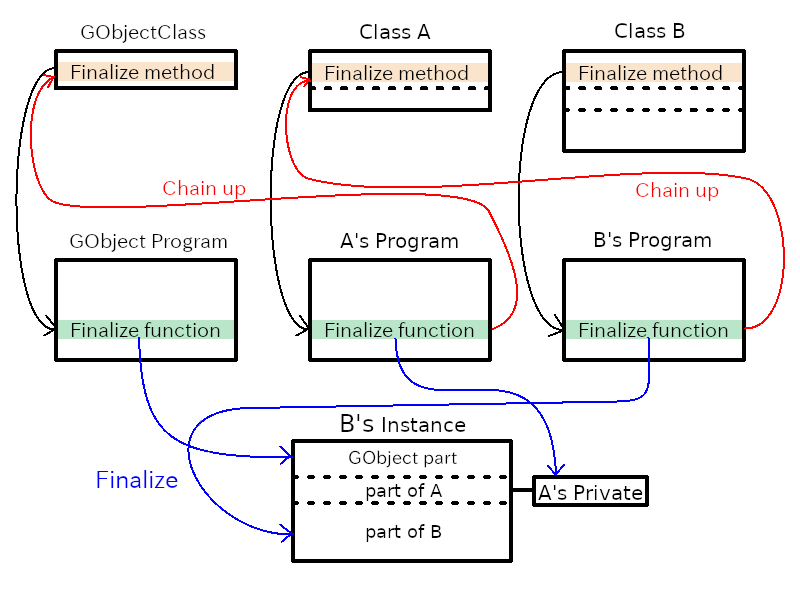
\includegraphics[width=12cm,height=9cm]{../image/chainup3.png}
\caption{Chaining up process}
\end{figure}

\subsection{How to write a derivable
type}\label{how-to-write-a-derivable-type}

\begin{itemize}
\tightlist
\item
  Use \passthrough{\lstinline!G\_DECLARE\_DERIVABLE\_TYPE!} macro in the
  header file. You need to write a macro like
  \passthrough{\lstinline!\#define T\_TYPE\_STR (t\_str\_get\_type ())!}
  before \passthrough{\lstinline!G\_DECLARE\_DERIVABLE\_TYPE!}.
\item
  Declare your class structure in the header file. The contents of the
  class are open to the descendants. Most of the members are class
  methods.
\item
  Use \passthrough{\lstinline!G\_DEFINE\_TYPE\_WITH\_PRIVATE!} in the C
  file. You need to define the private area before
  \passthrough{\lstinline!G\_DEFINE\_TYPE\_WITH\_PRIVATE!}. It is a C
  structure and the name is ``\textless object
  name\textgreater Private'' like ``TStrPrivate''.
\item
  Define class and instance initialization functions.
\end{itemize}
